\scanpage{58}
\figure{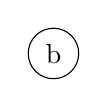
\begin{tikzpicture}\node[draw,circle] {b};\end{tikzpicture}}
\deleted{$\lambda_!\lambda^*(l_\bullet)\longrightarrow l_\bullet x$}

\deleted{$\lambda_!\lambda^*(l_\bullet)$ asphérique}
\deleted{$\unsure{Z^{(S)}}$}

(i) Si $l_\bullet$ \deleted{\unsure{réduit en degré $0$}},
\inserted{\unsure{hom} \unsure{acyclique}}, alors
$\lambda^*(l_\bullet)\deleted{\unsure{\otimes x}}\inserted{\otimes x}$
\deleted{\unsure{As}} \uline{acyclique}, pour \uline{tout $x$ [projectif]}

(ii) Si $l_\bullet$ est homotop. à $0$, alors $\lambda^*(l_\bullet)\otimes x$
acyclique pour tt $x$

(ii') $\lambda^*(\Theta_k)$ est acyclique.

(iii) $\deleted{\unsure{J\ Z}}\ \exists\ 1_M\xhookrightarrow{\alpha}J$
avec $\left\{\begin{array}{l}J\otimes x\text{ acyclique }\uline{\forall x\in M}\\
\alpha\otimes\mathrm{id}_x\text{ mono}\end{array}\right.$

\[
I\text{ asph sur }e\ \Longrightarrow\ J\deleted{\otimes}\otimes F\text{ acyclique}
\]
\[
\Longrightarrow\ \deleted{\unsure{Z^{(I)}\otimes F\longrightarrow F}}
\]
\[
\unsure{\in}\quad \unsure{\Longleftarrow}\quad
\unsure{\widetilde W_h^P(I)}\otimes F=\operatorname{Ker}(F^{(I)}\longrightarrow F)
\text{ est \deleted{asph} acyclique}
\]
\margin{donc $I\times X\mathbin{\text{---}}X$ équiv. faible pour tt. $X$.
$Z^{(I)}\times Z^{(X)}\longrightarrow Z^{(X)}$ équiv. faible \unsure{ab.}}

\uline{Lemme} Soit $I\in\operatorname{Ob}\widehat A$, asph. \deleted{sur} $e$.
Alors $\unsure{\widetilde W_h(I)}$ est \deleted{tot.} acyclique,
i.e. $\unsure{\widetilde W_h^P(I)}\otimes x$ est acyclique $\forall x$ dans $\widehat A$

a fortiori pour $x$ de la forme $Z^{(X)}$, ou $\unsure{Z^{(a)}}$
\[
\unsure{\widetilde W_h(I)}\otimes x\text{ est acyclique}
\]
\figure{\begin{tikzpicture}\draw (0,0)--(0.03,0.7)--(0.18,0.75);\end{tikzpicture}}

$J$ est $\otimes_M$-plat.

$J\otimes x$ acyclique pour $x$ projectif

$J\otimes x$ acyclique

\uline{Lemme} $J$ objet $\otimes_M$-plat. Conditions équivalentes

(i) $J\otimes_{\unsure{k}}x$ est \deleted{tot} acyclique pour tt $x$ dans $M$.

(ii) $J\otimes_{\unsure{k}}x\quad\rule{7cm}{0.3pt}\quad x$ projectif

i.e. $J$ est tot asph.

\uline{Corollaire} Car si c'est vrai

\figure{\begin{tikzpicture}\draw (0,0)--(5.8,0.55);\draw (6.2,0.62)--(13.2,0.8);\end{tikzpicture}}
\diagram{\begin{tikzcd}
l_\bullet\arrow[r] & l_\bullet\otimes\widetilde\Theta_k\arrow[l,bend left=55]
\end{tikzcd}}
\diagram{\begin{tikzcd}k\arrow[r]&\Theta_k\end{tikzcd}}
\diagram{\begin{tikzcd}l_\bullet\arrow[r,dash,shift left=2pt]\arrow[r,dash,shift right=2pt]&l'\end{tikzcd}}
\diagram{\begin{tikzcd}
l\otimes\Theta_k\arrow[r]&l'\\
l\arrow[u]&
\end{tikzcd}}
\mspage{57}
